\documentclass[11pt,a4paper]{article}
\usepackage[utf8]{inputenc}
\usepackage{geometry}
\geometry{top=2cm, bottom=2cm, left=2cm, right=2cm}
\usepackage{fancyhdr}
\usepackage{enumitem}
\usepackage{xcolor}
\usepackage{hyperref}
\usepackage{graphicx}
\usepackage{booktabs}
\usepackage{longtable}
\usepackage{titlesec}
\usepackage{float}

% Header and Footer
\pagestyle{fancy}
\fancyhf{}
\lhead{\textbf{Project Proposal}}
\rhead{\textbf{ID: EHPC-AIF-2026SC01-062}}
\cfoot{\thepage}

\title{\textbf{Project Proposal for Tier 0/Tier 1 HPC Access}}
\author{\textbf{Principal Investigator:} Jakub Mitura \\
\textbf{Affiliation:} Otto-von-Guericke University Magdeburg (OVGU) \\
\textbf{Contact:} jakub.mitura@ovgu.de}
\date{Period: April 2026 - March 2027}

\begin{document}

\maketitle
\thispagestyle{fancy}
\tableofcontents
\newpage

\section{Introduction}
\label{sec:intro}
\textbf{Objective:} To leverage advanced generative architectures—including but not limited to Diffusion Models, Variational Autoencoders (VAEs), and Transformers—to synthesize high-fidelity medical imagery (such as CT scans and dose maps) \cite{KazerouniAghdam2022, SanchezTsaftaris2022}. The project aims to enhance diagnostic precision while prioritizing patient safety.

\textbf{Context:} Nuclear Medicine involves the use of radioactive substances for diagnosis and therapy \cite{DulleaOSullivan2025}. Accurate dosimetry and high-quality anatomical references are crucial. This project addresses the scarcity of labeled medical data by using generative AI to create realistic synthetic datasets \cite{StauffenbergPoyet2024}, thereby improving the robustness of downstream AI tasks like segmentation and regression.

\section{Preliminary Work}
\label{sec:prelim}
We have performed extensive strong scaling tests on a single node with 8x NVIDIA H100 GPUs using a representative high-load architecture (Super Heavy 3D ResNet-152, 128x128x128 volume). The workload was compute-bound and memory-intensive, fully utilizing the 80GB HBM3 capacity per GPU (Batch Size 24).

We observed linear throughput scaling for our Julia (Lux.jl) implementation, achieving a 3.74x speedup on 4 GPUs (117.2 Samples/s) compared to 1 GPU (31.3 Samples/s). We also benchmarked a PyTorch implementation which showed good scaling but lower raw throughput on single GPU.

These benchmarks confirm that our hybrid infrastructure can effectively utilize the massive parallelism of the JUPITER Booster (NVIDIA GH200) for our proposed compute-intensive backbones.

\section{Description of the Project}
\label{sec:desc}

\subsection{Project Details}
\textbf{Scientific Goals:}
\begin{itemize}
    \item \textbf{Radiation Reduction:} Minimizing patient exposure by synthesizing high-quality diagnostic images from low-dose inputs.
    \item \textbf{Foundation Model Development:} Building scalable pre-trained models for diverse nuclear medicine tasks, including segmentation and regression.
    \item \textbf{Generative Augmentation:} Expanding limited medical datasets to improve the robustness of downstream AI tasks \cite{GoodfellowShlens2014}.
\end{itemize}

\textbf{Approach:}
We utilize a flexible modular framework for generative tasks. Our core methodologies include Generative Modeling (Diffusion, VAEs), Multi-Task Learning (simultaneous segmentation and reconstruction), and Generative Augmentation.

\textbf{Expected Impact:}
By integrating generative augmentation, we overcome the scarcity of labeled medical data, leading to more "generalizable" AI tools that perform reliably across different patient demographics and hardware.

\subsection{Review Processes}
Has the underlying research project already successfully undergone a scientific review process?
No, this is a new proposal for HPC access. The project is supported by public funding at Otto-von-Guericke University Magdeburg.

\section{Numerical Methods and Algorithms}
\label{sec:methods}
We employ a hybrid Julia/Python workflow designed for the JUPITER architecture.
\begin{itemize}
    \item \textbf{Julia (SciML):} Leveraging `EnsembleGPUArray` for massively parallel ODE solving and `KernelAbstractions.jl` for portable GPU kernels \cite{Li2023}. This allows for efficient simulation of physical processes using Neural ODEs \cite{ChenLiu2024}.
    \item \textbf{Python (PyTorch/Monai):} Utilizing `DistributedDataParallel` and `TorchDynamo` for efficient multi-node training of foundation models, particularly Transformers and CNNs.
    \item \textbf{Interoperability:} Seamless data exchange via `PythonCall.jl` and `DLPack` combines the best-in-class differential equation solvers from Julia with the rich deep learning ecosystem of Python.
\end{itemize}

\section{Computer Resources}
\label{sec:resources}

\subsection{Code performance and workflow}
The application is compute-bound during training and potentially I/O bound during data loading, addressed by our HDF5 strategy.
We present the scaling behavior of our code (Lux.jl) on NVIDIA H100 GPUs (comparable architecture to JUPITER Booster) in Table \ref{tab:scaling} and Figure \ref{fig:scaling}.

\begin{table}[h]
\centering
\caption{Scaling behavior of Lux.jl on NVIDIA H100 GPU Cluster. Problem size: 128x128x128 3D Volume (ResNet-152).}
\label{tab:scaling}
\begin{tabular}{ccc}
\toprule
\# GPUs & Throughput (Samples/s) & Speedup \\
\midrule
1 & 31.3 & 1.0 \\
2 & 61.4 & 1.96 \\
4 & 117.2 & 3.74 \\
\bottomrule
\end{tabular}
\end{table}

\begin{figure}[H]
\centering
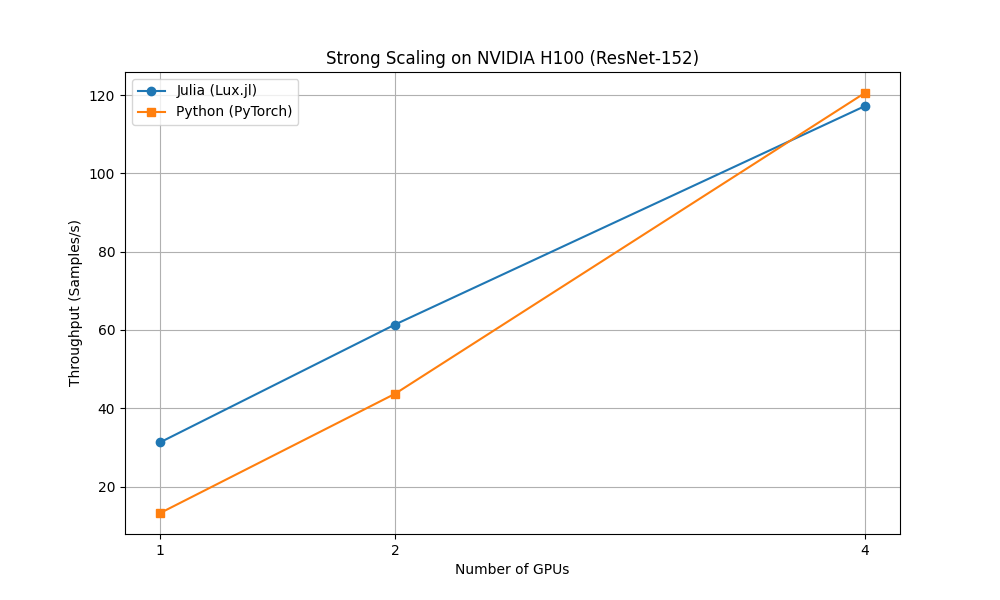
\includegraphics[width=0.8\textwidth]{scaling_plot.png}
\caption{Scaling behavior of Lux.jl vs PyTorch on H100 GPUs.}
\label{fig:scaling}
\end{figure}

\textbf{Memory Requirements:} The workload requires significant GPU memory (approx. 75-80GB per GPU for batch size 24). JUPITER Booster nodes with 4x GH200 (96GB HBM3 each) are ideal for this workload.

\textbf{I/O Strategy:} We use HDF5 with MPI-IO drivers (via HDF5.jl and h5py) to enable parallel reading/writing of large 3D volumes (approx. 300 TB total dataset size) and checkpoints across multiple nodes.

\subsection{Justification of resources requested}
We request a total of \textbf{100,000 GPU Hours} on JUPITER Booster (FZJ).
The project involves training multiple generative models (VAEs, Diffusion) and foundation models.
Assuming a typical job uses 4 GPUs (1 node) and runs for 5.75 hours (to fit within queue limits and checkpointing), we plan for approximately 4,350 job runs over the year.

\begin{table}[h]
\centering
\caption{The following GPU resources are requested}
\label{tab:gpu_resources}
\resizebox{\textwidth}{!}{%
\begin{tabular}{lcccccccc}
\toprule
Sub-project & Type of run & Problem size & \# runs & \# steps/run & Wall time/step [h] & \# GPUs/run & \# host cores/run & Total [GPU-h] \\
\midrule
GenAI-Med & Production & 128$^3$ & 4,350 & 1 & 5.75 & 4 & 288 & 100,050 \\
\midrule
\textbf{TOTAL} & & & & & & & & \textbf{100,050} \\
\bottomrule
\end{tabular}%
}
\end{table}

\section{Resource Management and Work Schedule}
\label{sec:management}

\subsection{Resource management}
We will use a detailed logging system to monitor job execution and resource utilization. Checkpoints are written every 2-4 hours to ensure progress is saved. Data is stored on SCRATCH (300 TB quota requested) and archived appropriately.

\subsection{Work schedule}
The project follows a phased approach:
\begin{enumerate}
    \item \textbf{Profiling \& Porting (M1-M2):} Adapting code to Grace-Hopper architecture.
    \item \textbf{Scaling Tests (M3-M4):} Weak/Strong scaling to larger node counts.
    \item \textbf{Production Training \& Exploration (M5-M12):} Full-scale training of foundation models.
\end{enumerate}

See Figure \ref{fig:gantt} for the Gantt chart.

\begin{figure}[H]
\centering
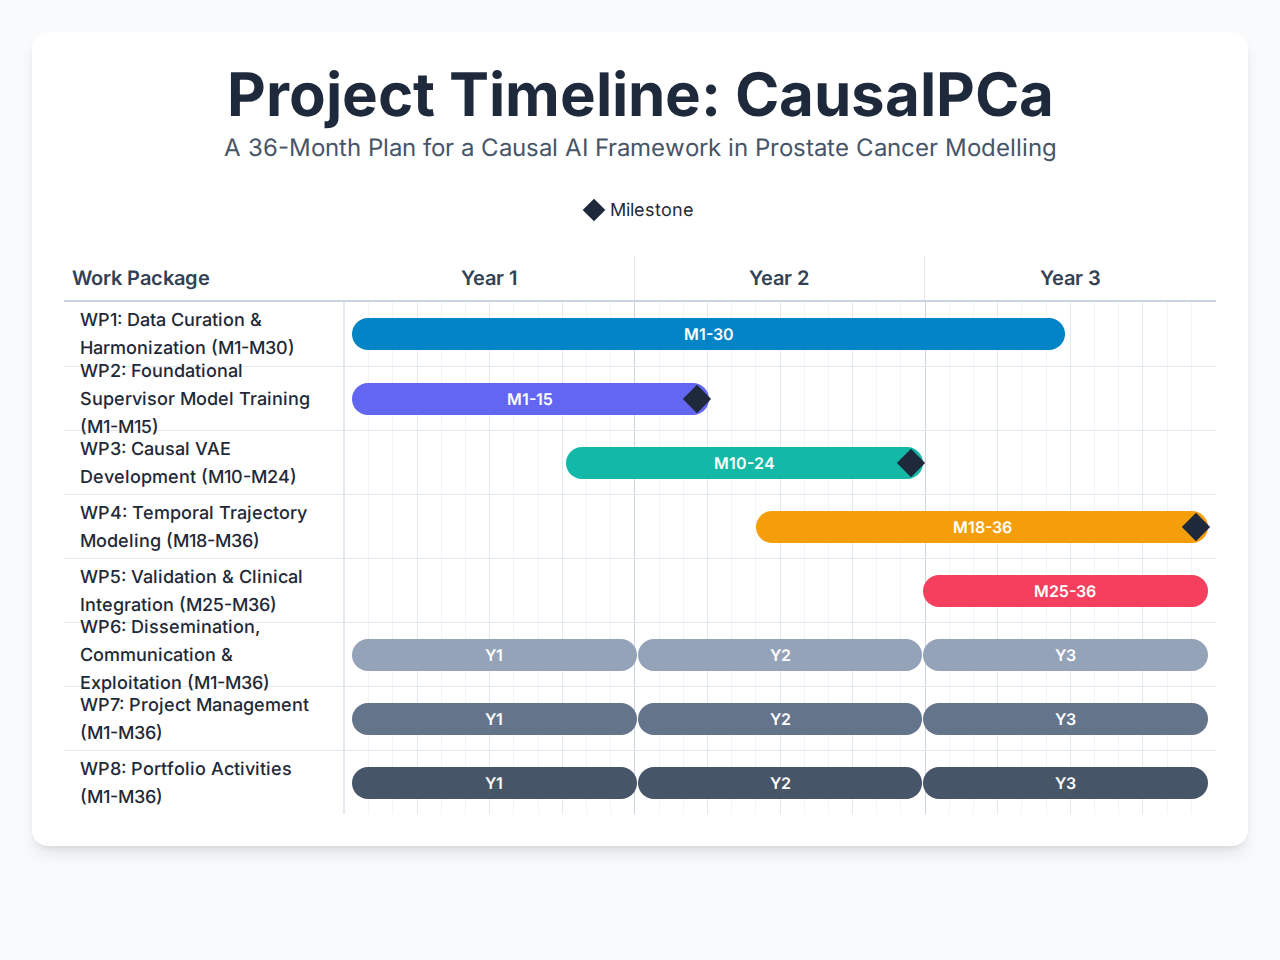
\includegraphics[width=1.0\textwidth]{../gantt.png}
\caption{Work schedule for the project.}
\label{fig:gantt}
\end{figure}

\section{Key Personnel and Experiences}
\label{sec:personnel}
\begin{itemize}
    \item \textbf{Jakub Mitura (PI):} Expertise in Deep Learning and Medical Imaging. Responsible for overall project management and model architecture.
    \item \textbf{Joanna Wybrańska:} Experience in data preprocessing and clinical validation.
    \item \textbf{Medical Faculty of OVGU Team:} Domain experts providing clinical context and data.
\end{itemize}

\section{Bibliographic References}
\bibliographystyle{plain}
\bibliography{references}

\end{document}
